\documentclass[UTF8,a4paper,11pt]{ctexart}
\usepackage[a4paper,margin=2.2cm]{geometry}
\usepackage{booktabs}
\usepackage{array}
\usepackage{longtable}
\usepackage{graphicx}
\usepackage{caption}
\usepackage{float}
\usepackage{placeins}
\usepackage{enumitem}
\usepackage{xcolor}
\usepackage{tikz}
\usepackage{pgfplots}
\pgfplotsset{compat=1.18}
\usepgfplotslibrary{groupplots}
\definecolor{PFullColor}{RGB}{31,78,140}
\definecolor{PMinColor}{RGB}{88,145,201}
\definecolor{PNatColor}{RGB}{166,199,231}
\definecolor{TFullColor}{RGB}{184,88,18}
\definecolor{TMinColor}{RGB}{224,150,70}
\definecolor{TNatColor}{RGB}{246,199,146}
\usepackage[hidelinks]{hyperref}

\setlist{nosep,leftmargin=2em}
\captionsetup{font=small,labelfont=bf}
\title{Minecraft 服务端 Agent 部署方式对比实验报告}
\author{实验记录整理稿}
\date{2026 年 10 月 22 日}

\newcommand{\mctfull}{\texttt{MCT-full}}
\newcommand{\mctminimal}{\texttt{MCT-minimal}}
\newcommand{\ocminimal}{\texttt{Opencode-minimal}}
\newcommand{\pixelmon}{Pixelmon}
\newcommand{\twilight}{Twilight Forest}

\begin{document}
\maketitle

\begin{abstract}
本文比较三种 Minecraft 服务端自动部署方式在两个真实整合包服务端上的表现：完整的 MCT Agent（包含流程编排与 DAG 依赖图）、精简的 MCT Agent（basic 模式，不启用 DAG 编排）以及使用原生工具的 OpenCode Agent。实验共包含两个服务端、三种方式、六次独立部署。结果表明，完整 MCT 在外部可靠性上最稳定，两个服务端均通过 8 项外部检查；精简 MCT 在 Pixelmon 上耗时最低，但在 Twilight Forest 上出现配置项未通过；原生 OpenCode 在两个样本中都产生较高的工具负担，其中 Pixelmon 未完成有效启动验收，Twilight Forest 虽通过外部状态检查但超过任务时限。由于每个条件只有一次观测，本文将结果解释为探索性证据，不进行显著性或稳定平均效果推断。
\end{abstract}

\section{实验目标}

\subsection{研究背景与问题}
Minecraft 服务端部署不是单一文件复制任务，而是包含整合包识别、Java 版本判断、服务端包准备、Loader 安装、Python 与 MCDReforged 配置、进程启动以及外部状态验证的一组有依赖关系的操作。不同 Agent 方案在工具抽象、流程约束和验证闭环上的差异，可能导致显著不同的可靠性和端到端耗时。

本实验围绕以下研究问题展开：
\begin{enumerate}
  \item \textbf{RQ1：}完整的领域工具链与 DAG 流程编排是否能提高部署的外部可靠性？
  \item \textbf{RQ2：}去除完整流程编排、仅保留 basic 工具能力后，是否能够降低模型交互成本并保持部署质量？
  \item \textbf{RQ3：}仅使用原生文件与 Shell 工具的 OpenCode Agent，能否在复杂整合包上稳定完成部署并及时收束？
  \item \textbf{RQ4：}不同服务端复杂度是否会改变三种部署方式的相对表现？
\end{enumerate}

\subsection{待验证假设}
\begin{description}
  \item[H1（可靠性）] 完整 MCT 的领域工具、DAG 依赖和外部验证闭环能够使关键外部检查通过率高于两种精简或原生方式。
  \item[H2（效率）] MCT 的专用工具能够减少模型反复试错，因此端到端部署耗时和工具错误数低于原生 OpenCode。
  \item[H3（精简权衡）] \mctminimal{} 由于不启用 DAG 和完整流程提示，可能减少模型步骤和输出 Token，但其可靠性可能因缺少流程约束而下降。
  \item[H4（复杂度交互）] 服务端包的结构、Loader 安装难度和运行时依赖会调节部署方式的效果，因此不能只用单一服务端得出结论。
\end{description}

\subsection{为什么进行该实验}
本实验的目的不是证明某一 Agent 在所有任务上绝对优越，而是建立一个可审计的工程基线：明确领域编排、精简编排和原生工具操作之间的性能与可靠性代价，为后续是否保留 DAG、如何改造持续执行机制以及如何设计部署验收边界提供数据依据。

\section{实验设置}

\subsection{数据集与实验单元}
实验采用原始服务端矩阵中已经确定的两个服务端，每个服务端在三种条件下各运行一次，共六个独立实验单元。服务端输入、版本和包格式如下。

\begin{table}[H]
\centering
\caption{实验输入与环境基线}
\label{tab:setup}
\small
\begin{tabular}{lll}
\toprule
项目 & \pixelmon{} & \twilight{} \\
\midrule
服务端包 & serverpack9314.zip & twilight-forest-1.0.zip \\
包版本 & 9.3.14 & 1.0 \\
Minecraft & 1.21.1 & 1.21.1 \\
Loader & NeoForge & NeoForge \\
包格式 & 完整 server pack & 完整 server pack \\
模型 & \multicolumn{2}{l}{deepseek-v4-flash-vision-exp，high reasoning} \\
内存上限 & \multicolumn{2}{l}{3584 MiB（Xms = Xmx = 3584M）} \\
运行时基线 & \multicolumn{2}{l}{相同 Java / Python baseline 与代理} \\
模板 & \multicolumn{2}{l}{相同原始 MCDR 模板} \\
隔离方式 & \multicolumn{2}{l}{全新 workspace，独立端口，串行运行} \\
\bottomrule
\end{tabular}
\par\smallskip
{\footnotesize 注：完整包名为 serverpack9314.zip 与 The-Best-of-Twilight-Forest-Server-1.0.zip。}
\end{table}

\subsection{对照方法}
\begin{table}[H]
\centering
\caption{三种部署方式的操作定义}
\label{tab:conditions}
\small
\begin{tabular}{p{0.22\textwidth}p{0.69\textwidth}}
\toprule
条件 & 定义 \\
\midrule
\mctfull{} & MCT 完整 Agent；使用领域专用工具、完整系统提示、Skills、DAG 步骤依赖、后台 Job 与外部验证。拓扑层用于表达依赖和并行关系。 \\
\mctminimal{} & MCT basic benchmark 模式；保留 MCT 受控工具和生命周期管理，但不注册 \texttt{begin\_deployment\_workflow} 与 \texttt{update\_agent\_workflow\_progress}，不加载完整 DAG 流程。 \\
\ocminimal{} & OpenCode 原生工具模式；使用最小系统提示和原生文件/Shell 工具，不使用 MCT 专用部署面板、DAG 或额外 Skills，并隔离 HOME 与配置。 \\
\bottomrule
\end{tabular}
\end{table}

\subsection{评测指标}
\begin{enumerate}
  \item \textbf{端到端耗时：}从部署 CLI 启动到 CLI 退出，单位为秒；准备、外部评测、LLM 评分、停服和归档不计入部署 wall time。
  \item \textbf{模型交互：}模型请求数、执行步骤数、原始 prompt 与 completion tokens。
  \item \textbf{工具行为：}工具调用数、工具错误数、工具活跃时间并集，以及流程进度调用和验证调用。
  \item \textbf{外部可靠性：}八项二值检查，包括 MCDR 配置、MCDR 启动接管、插件加载、Minecraft 启动、Minecraft 状态响应、隔离监听、安全配置和内存限制。
  \item \textbf{任务状态：}\texttt{completed}、\texttt{timed\_out} 或 \texttt{cli\_exited}；状态不以模型最终文字代替外部事实。
  \item \textbf{可复现性与清理：}正常停服、进程和端口释放、workspace 归档可读性及 SHA-256 校验。
  \item \textbf{辅助质量指标：}独立 LLM 评分仅作为次要主观指标，不计入部署时间和部署 Token，也不替代外部验收。
\end{enumerate}

\subsection{说服力与控制措施}
实验采用固定模型、固定推理强度、固定内存、固定 Java/Python baseline、固定代理和固定模板；每个条件使用独立 workspace，运行过程串行并通过锁避免并发；原始包、模板和执行源码记录 SHA-256；部署成功与否由独立进程、端口、Minecraft 协议响应、日志和配置检查共同判定；停止服务只通过当前试验拥有的 API 或已验证的 MCDR 输入执行，不自动强杀。

需要强调的是，本实验每个条件只有一次观测，且条件顺序固定，无法估计方差、置信区间或统计显著性。它是工程系统比较和机制筛选，而不是严格的随机对照试验。

\section{实验结果}

\subsection{核心结果}
\begin{table}[H]
\centering
\caption{六次部署实验的核心结果（三线表）}
\label{tab:main-results}
\scriptsize
\resizebox{\textwidth}{!}{%
\begin{tabular}{llrrrrrrrr}
\toprule
服务端 & 条件 & 状态 & 耗时(s) & 请求/步骤 & 输出 Token & Tool(s) & 工具数 & 错误 & 外部检查 \\
\midrule
\pixelmon{} & \mctfull{} & completed & 526.168 & 65/65 & 34,548 & 282.626 & 82 & 2 & 8/8 \\
\pixelmon{} & \mctminimal{} & completed & 402.760 & 36/36 & 12,764 & 302.038 & 47 & 1 & 8/8 \\
\pixelmon{} & \ocminimal{} & cli\_exited & 1,480.660 & 68/66 & 37,006 & 1,275.731 & 80 & 4 & 3/8 \\
\twilight{} & \mctfull{} & completed & 220.663 & 27/27 & 16,064 & 113.204 & 38 & 0 & 8/8 \\
\twilight{} & \mctminimal{} & completed & 513.790 & 72/72 & 37,207 & 229.742 & 111 & 3 & 7/8 \\
\twilight{} & \ocminimal{} & timed\_out & 1,900.466 & 105/103 & 63,701 & 1,399.420 & 118 & 3 & 8/8 \\
\bottomrule
\end{tabular}
}%
\end{table}

\subsection{耗时与可靠性图表}
图 \ref{fig:metrics-p} 和图 \ref{fig:metrics-t} 按服务端分为两张图，各含十项指标，图内标签统一使用英文。由于量纲不同，两图统一以 Pixelmon \mctfull{} 的对应指标为 100\% 换算为相对值，并采用相同纵轴范围，可直接比较。

\begin{figure}[H]
\centering
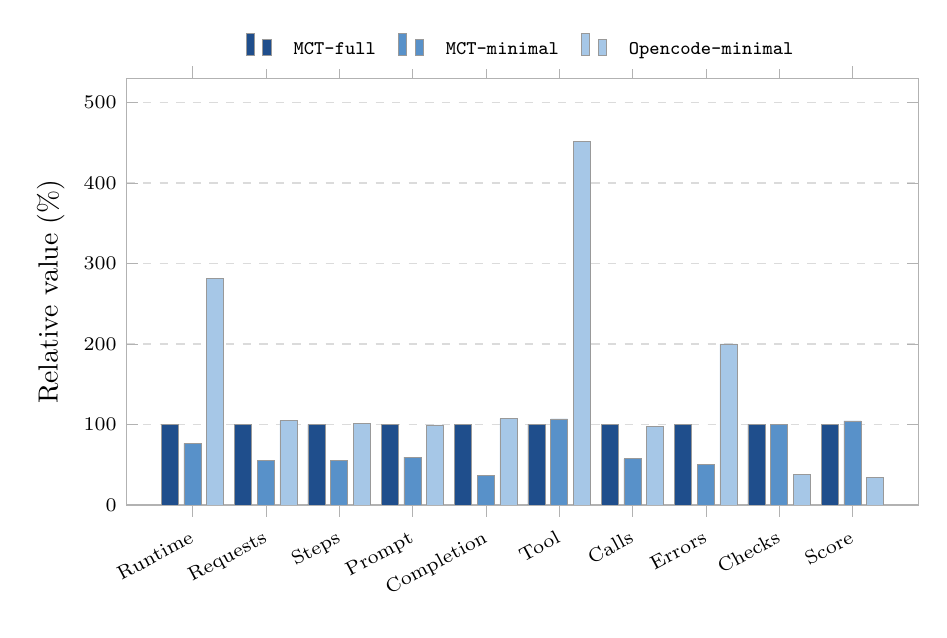
\begin{tikzpicture}
\begin{axis}[
  ybar,
  /pgf/bar width=6.2pt,
  width=0.96\textwidth,
  height=7cm,
  ymin=0,
  ymax=530,
  ylabel={Relative value (\%)},
  symbolic x coords={Runtime,Requests,Steps,Prompt,Completion,Tool,Calls,Errors,Checks,Score},
  xtick={Runtime,Requests,Steps,Prompt,Completion,Tool,Calls,Errors,Checks,Score},
  xticklabel style={font=\scriptsize,rotate=28,anchor=north east},
  yticklabel style={font=\scriptsize},
  ymajorgrids=true,
  grid style={dashed,gray!28},
  axis line style={gray!60},
  tick style={gray!60},
  enlarge x limits=0.1,
  legend style={at={(0.5,1.02)},anchor=south,legend columns=3,draw=none,font=\scriptsize,column sep=6pt,inner sep=2pt},
  every axis plot/.append style={line width=0.25pt}
]
\addplot[fill=PFullColor,draw=black!40,line width=0.25pt] coordinates {(Runtime,100.0) (Requests,100.0) (Steps,100.0) (Prompt,100.0) (Completion,100.0) (Tool,100.0) (Calls,100.0) (Errors,100.0) (Checks,100.0) (Score,100.0)};
\addplot[fill=PMinColor,draw=black!40,line width=0.25pt] coordinates {(Runtime,76.5) (Requests,55.4) (Steps,55.4) (Prompt,59.4) (Completion,36.9) (Tool,106.9) (Calls,57.3) (Errors,50.0) (Checks,100.0) (Score,104.3)};
\addplot[fill=PNatColor,draw=black!40,line width=0.25pt] coordinates {(Runtime,281.4) (Requests,104.6) (Steps,101.5) (Prompt,99.4) (Completion,107.1) (Tool,451.4) (Calls,97.6) (Errors,200.0) (Checks,37.5) (Score,34.4)};
\legend{\mctfull{},\mctminimal{},\ocminimal{}}
\end{axis}
\end{tikzpicture}
\caption{Relative metrics on Pixelmon, normalized to \mctfull{} (all bars at 100\%).}
\label{fig:metrics-p}
\end{figure}

\begin{figure}[H]
\centering
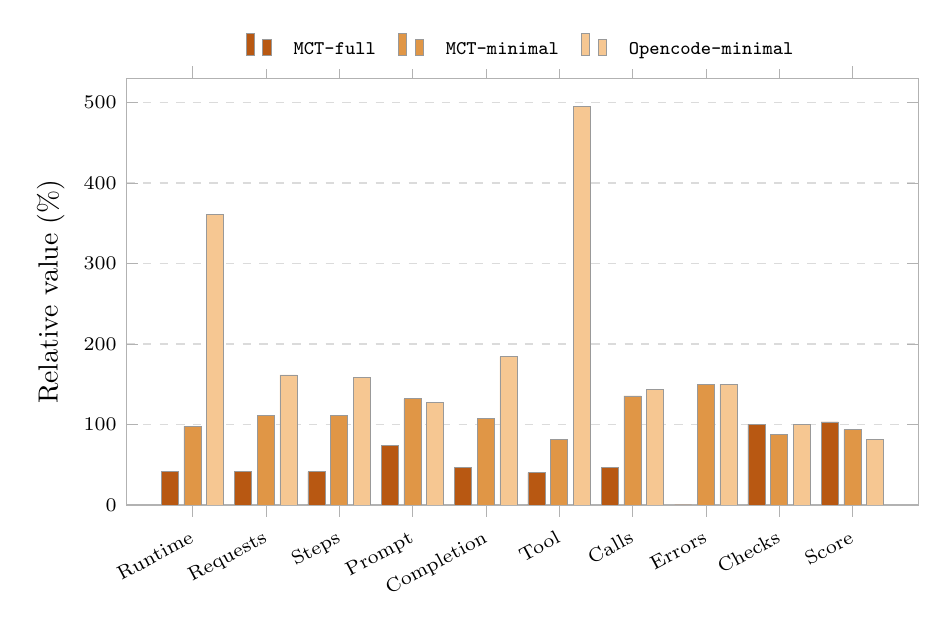
\begin{tikzpicture}
\begin{axis}[
  ybar,
  /pgf/bar width=6.2pt,
  width=0.96\textwidth,
  height=7cm,
  ymin=0,
  ymax=530,
  ylabel={Relative value (\%)},
  symbolic x coords={Runtime,Requests,Steps,Prompt,Completion,Tool,Calls,Errors,Checks,Score},
  xtick={Runtime,Requests,Steps,Prompt,Completion,Tool,Calls,Errors,Checks,Score},
  xticklabel style={font=\scriptsize,rotate=28,anchor=north east},
  yticklabel style={font=\scriptsize},
  ymajorgrids=true,
  grid style={dashed,gray!28},
  axis line style={gray!60},
  tick style={gray!60},
  enlarge x limits=0.1,
  legend style={at={(0.5,1.02)},anchor=south,legend columns=3,draw=none,font=\scriptsize,column sep=6pt,inner sep=2pt},
  every axis plot/.append style={line width=0.25pt}
]
\addplot[fill=TFullColor,draw=black!40,line width=0.25pt] coordinates {(Runtime,41.9) (Requests,41.5) (Steps,41.5) (Prompt,73.9) (Completion,46.5) (Tool,40.1) (Calls,46.3) (Errors,0.0) (Checks,100.0) (Score,103.2)};
\addplot[fill=TMinColor,draw=black!40,line width=0.25pt] coordinates {(Runtime,97.6) (Requests,110.8) (Steps,110.8) (Prompt,131.9) (Completion,107.7) (Tool,81.3) (Calls,135.4) (Errors,150.0) (Checks,87.5) (Score,93.5)};
\addplot[fill=TNatColor,draw=black!40,line width=0.25pt] coordinates {(Runtime,361.2) (Requests,161.5) (Steps,158.5) (Prompt,127.0) (Completion,184.4) (Tool,495.1) (Calls,143.9) (Errors,150.0) (Checks,100.0) (Score,81.7)};
\legend{\mctfull{},\mctminimal{},\ocminimal{}}
\end{axis}
\end{tikzpicture}
\caption{Relative metrics on Twilight Forest, using the same baseline and scale as Fig.~\ref{fig:metrics-p}.}
\label{fig:metrics-t}
\end{figure}

图内指标依次为端到端耗时、模型请求数、模型步骤数、Prompt Token、Completion Token、工具活跃时间、工具调用数、工具错误数、外部检查通过率和 LLM 评分。检查项低于 100\% 表示通过率下降；Pixelmon \ocminimal{} 为 37.5\%，对应 3/8。通过率不等同于完整功能验收。

\subsection{模型与工具开销}
\begin{table}[H]
\centering
\caption{模型请求、工具负担和辅助评分（三线表）}
\label{tab:overhead}
\small
\resizebox{\textwidth}{!}{%
\begin{tabular}{llrrrrrr}
\toprule
服务端 & 条件 & 模型请求 & 模型步骤 & Prompt Token & Completion Token & 工具错误 & LLM 评分 \\
\midrule
\pixelmon{} & \mctfull{} & 65 & 65 & 82,853 & 34,548 & 2 & 93 \\
\pixelmon{} & \mctminimal{} & 36 & 36 & 49,174 & 12,764 & 1 & 97 \\
\pixelmon{} & \ocminimal{} & 68 & 66 & 82,385 & 37,006 & 4 & 32 \\
\twilight{} & \mctfull{} & 27 & 27 & 61,194 & 16,064 & 0 & 96 \\
\twilight{} & \mctminimal{} & 72 & 72 & 109,250 & 37,207 & 3 & 87 \\
\twilight{} & \ocminimal{} & 105 & 103 & 105,245 & 63,701 & 3 & 76 \\
\bottomrule
\end{tabular}
}%
\end{table}

\subsection{按部署方式的两样本均值}
\begin{table}[H]
\centering
\caption{按部署方式汇总的两服务端均值；仅作描述性统计（三线表）}
\label{tab:means}
\small
\begin{tabular}{lrrrrrr}
\toprule
条件 & 耗时(s) & 模型请求 & 模型步骤 & 输出 Token & 工具调用 & 工具错误 \\
\midrule
\mctfull{} & 373.416 & 46.0 & 46.0 & 25,306 & 60.0 & 1.0 \\
\mctminimal{} & 458.275 & 54.0 & 54.0 & 24,986 & 79.0 & 2.0 \\
\ocminimal{} & 1,690.563 & 86.5 & 84.5 & 50,354 & 99.0 & 3.5 \\
\bottomrule
\end{tabular}
\end{table}

\section{结果分析}

\subsection{主要现象与解释}
\paragraph{完整 MCT 的可靠性最稳定。}
\mctfull{} 在两个服务端均达到 8/8 外部检查，且 Twilight Forest 上以 220.663 秒完成，是六个样本中最快的正常完成记录。其优势来自专用工具对 Java、Loader、MCDR、启动、停服和验证的封装，以及 DAG 对步骤依赖和并行关系的显式表达，降低了模型自行猜测命令和路径的空间。

\paragraph{精简 MCT 的收益依赖服务端。}
在 Pixelmon 上，\mctminimal{} 只耗时 402.760 秒，较 \mctfull{} 少 23.45\%，同时模型步骤从 65 降至 36、输出 Token 从 34,548 降至 12,764，且仍达到 8/8。另一方面，在 Twilight Forest 上，\mctminimal{} 耗时 513.790 秒，较 \mctfull{} 慢 132.82\%，模型步骤增加到 72，工具调用增加到 111，并且 MCDR 配置检查未通过。说明去掉 DAG 和完整部署提示可以减少固定提示负担，但也可能将流程控制成本转移给模型的试错和重复调用。

\paragraph{原生 OpenCode 的工具轨迹明显更重。}
\ocminimal{} 在 Pixelmon 上以 \texttt{cli\_exited} 结束，仅通过 3/8 检查且清理未通过；在 Twilight Forest 上虽然通过 8/8 外部检查，但消耗 103 个模型步骤、118 次工具调用，并超过 1800 秒任务上限。原生方式缺乏 MCT 的领域工具和流程收束机制，模型需要自行处理目录、安装器、启动命令和验证闭环，因而更容易出现重复检查、路径修复和长时间工具等待。

\paragraph{外部状态与任务状态必须分开。}
Twilight Forest 的 \ocminimal{} 是典型例子：外部服务端最终运行正常，但 Agent 任务状态是 \texttt{timed\_out}。相反，Pixelmon 的 \ocminimal{} 任务退出时并未形成有效的完整外部验收。因而“服务器启动过”不能直接等价于“部署任务成功”，必须同时报告任务生命周期、外部检查和清理证据。

\subsection{对研究问题和假设的回答}
\begin{itemize}
  \item 对 RQ1：在本实验样本中，完整 MCT 的外部可靠性最好，两个服务端均为 8/8，初步支持 H1。
  \item 对 RQ2：\mctminimal{} 在 Pixelmon 上显著减少模型交互并保持 8/8，但在 Twilight Forest 上出现 7/8 和更高交互负担，H3 仅得到条件性支持。
  \item 对 RQ3：原生 OpenCode 在两个服务端均表现出更高的步骤、工具和耗时负担；一个超时、一个 CLI 退出，不能支持其在本实验设置下稳定完成复杂部署。
  \item 对 RQ4：两服务端的排序不同，说明服务端复杂度和包内安装路径确实会调节部署方式表现，支持 H4。
\end{itemize}

\subsection{局限性}
\begin{enumerate}
  \item 每个条件只有一次观测，无法估计随机波动、置信区间或显著性；结果只能作为探索性比较。
  \item 条件按固定顺序串行运行，文件系统、网络和模型缓存可能产生顺序效应。
  \item 两个服务端不足以代表 Minecraft 整合包总体，尤其不能覆盖 Fabric、Quilt、无官方 server pack 或不同规模的服务端。
  \item LLM 评分是独立模型请求产生的主观辅助指标，不应当替代外部验收。该样本首次评审未返回有效 JSON，分数来自同一评估函数对同一证据的重评。
  \item 外部检查覆盖启动、配置、插件加载和协议状态，但不覆盖玩家登录、完整游戏玩法、插件业务功能和真实 ChatHub 远程服务。
  \item 上游 usage 的 prompt、total 和 cache 字段口径不一致，不能从观测 cache hit 倒推出真实输入量或成本。
\end{enumerate}

\subsection{改进方向}
\begin{enumerate}
  \item 将每个条件扩展为至少 3 次重复，并随机化条件顺序；报告均值、标准差和置信区间。
  \item 将 DAG 的贡献与领域工具贡献拆开做正交消融，例如保留专用工具但去除 DAG、保留 DAG 但限制工具抽象，避免把多个机制混为一个条件。
  \item 为原生 OpenCode 增加统一的任务完成边界、后台任务等待和外部验收接口，再比较“工具能力差异”而不是“工具能力加收束机制差异”。
  \item 将模型步骤、工具等待、文件解压、Loader 安装、Minecraft 启动和停服等待拆成可比较的阶段时间，并记录每阶段的重试和失败原因。
  \item 修复 usage 网关的缓存字段语义，使输入 Token、缓存命中和成本能够按统一协议计算。
  \item 扩展服务端样本，覆盖 Fabric/Quilt、manifest 组装包、轻量包和大型包，并加入玩家连接与核心插件功能的独立验收。
\end{enumerate}

\enlargethispage{3\baselineskip}
\section*{数据与复现说明}
原始六次结果位于 \texttt{exp/the-pixelmon-modpack/} 与 \texttt{exp/the-best-of-twilight-forest/}，汇总文件为 \texttt{exp/results.csv} 和 \texttt{exp/results.json}；实验协议见 \texttt{scripts/benchmark-suite.md}。后续单次持续执行的 Pixelmon 工程版验收不纳入本文主结果。

\end{document}
